\documentclass{article}
\usepackage[paperwidth=30cm,paperheight=13.8cm,margin=0.6cm]{geometry}
\usepackage{fontspec}
\setmainfont{texgyreheros}[Extension=.otf,UprightFont=*-regular,BoldFont=*-bold,ItalicFont=*-italic,BoldItalicFont=*-bolditalic]
\usepackage{xcolor}
\usepackage{tikz}
\usetikzlibrary{arrows.meta,positioning,calc,backgrounds,fit}
\pagestyle{empty}

\definecolor{ink}{HTML}{14213D}
\definecolor{grey}{HTML}{6B7280}
\definecolor{bankc}{HTML}{1F6F8B}
\definecolor{keyc}{HTML}{8E2C6E}
\definecolor{user}{HTML}{2F7A4F}
\definecolor{gold}{HTML}{9A6B00}
\definecolor{softgold}{HTML}{FBF3DC}
\definecolor{softblue}{HTML}{E6EEF8}
\definecolor{softgreen}{HTML}{E4F1E8}
\definecolor{softgrey}{HTML}{F1F2F4}
\definecolor{softkey}{HTML}{F4E6EF}

\newcommand{\num}[1]{\tikz[baseline=(c.base)]\node[circle,fill=ink,text=white,inner sep=1.2pt,font=\bfseries\small] (c) {#1};}
\newcommand{\new}[1]{\tikz[baseline=(c.base)]\node[fill=softgold,draw=gold,text=gold,rounded corners=1pt,inner sep=1.5pt,font=\bfseries\footnotesize] (c) {#1};}

\tikzset{
  actor/.style={draw=#1,fill=white,line width=1.2pt,rounded corners=4pt,inner sep=7pt,align=left,text width=5.6cm,font=\small},
  head/.style={font=\bfseries\large},
  flow/.style={-{Stealth[length=3mm]},line width=1.1pt,draw=ink},
  lab/.style={font=\small,align=left,fill=white,inner sep=2pt},
}

\begin{document}
\centering
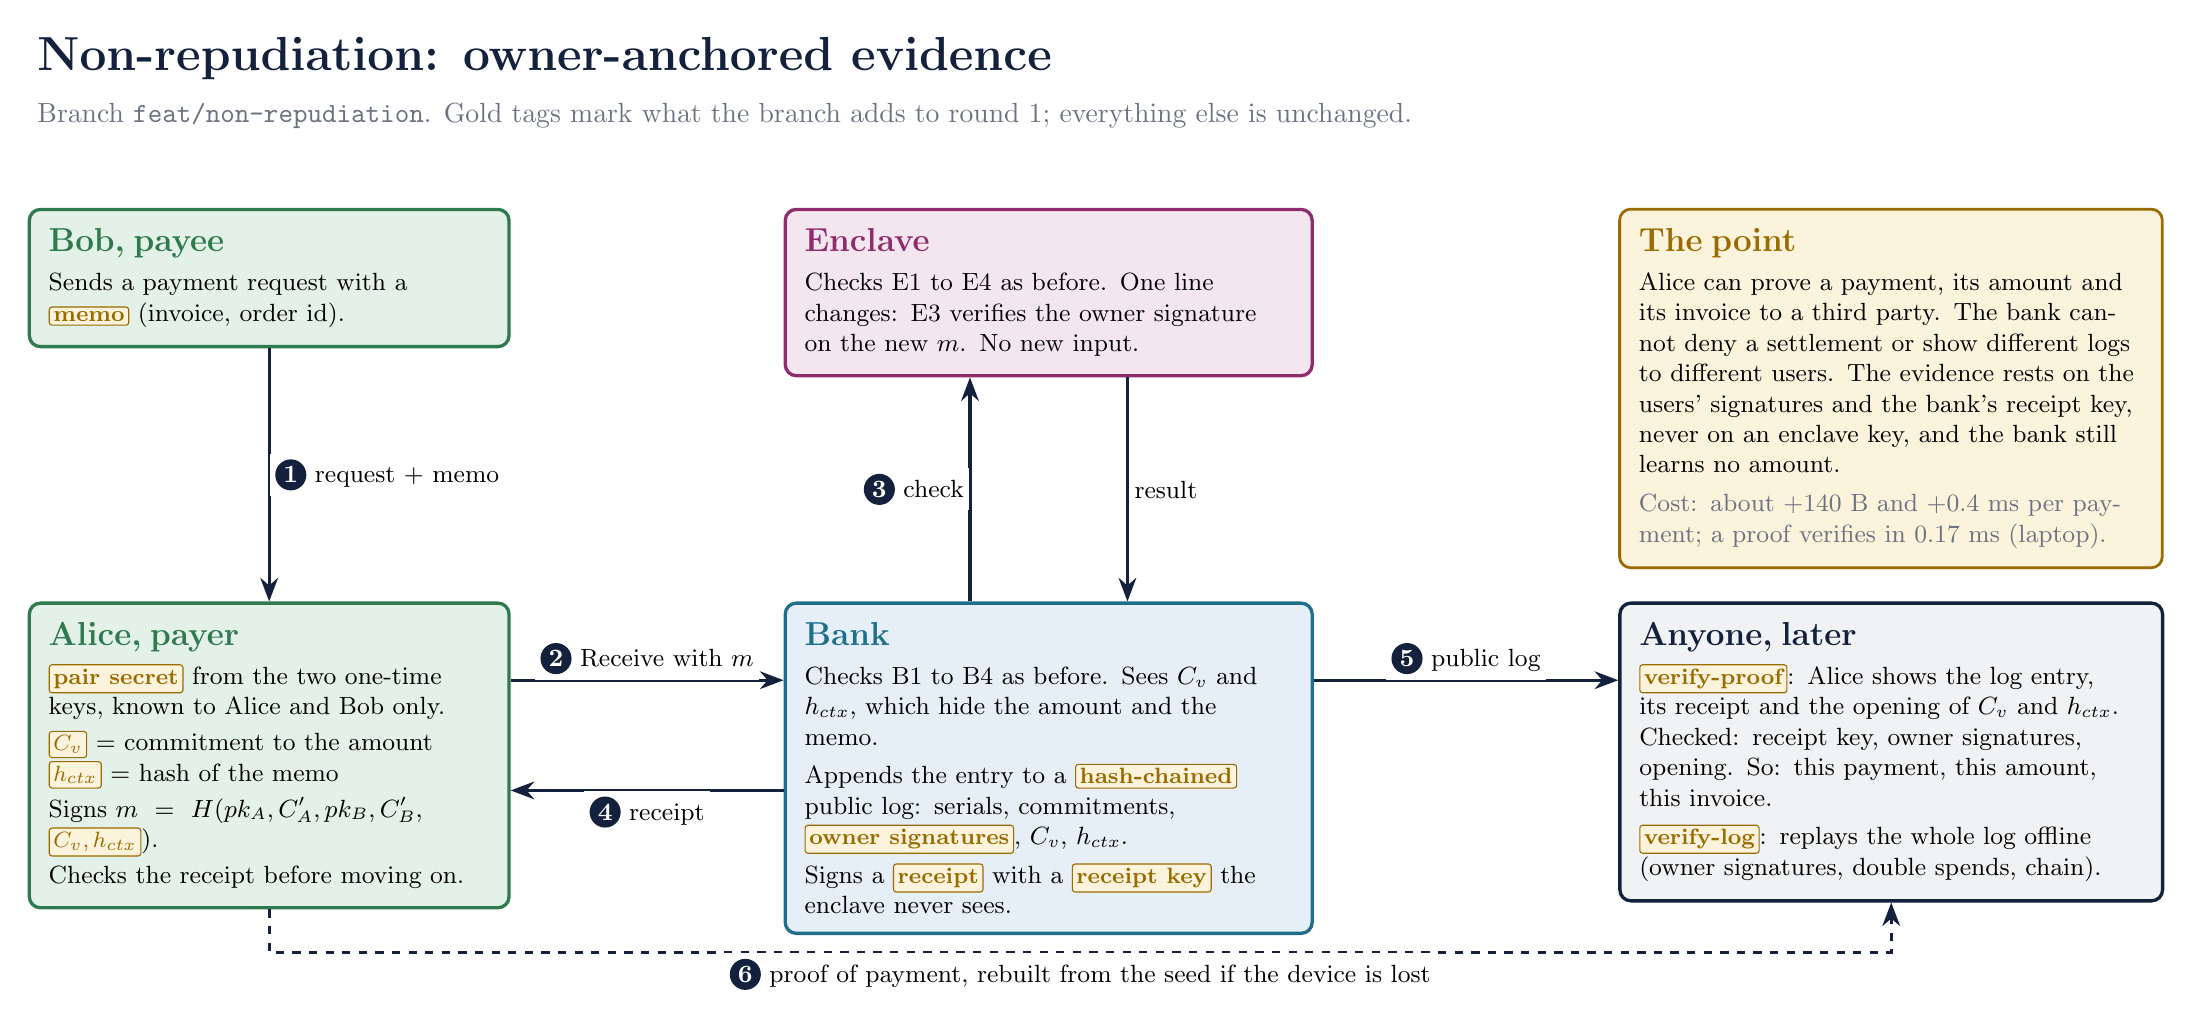
\begin{tikzpicture}[node distance=1.2cm]

\node[font=\bfseries\LARGE,text=ink,anchor=west] (title) at (0,0) {Non-repudiation: owner-anchored evidence};
\node[font=\normalsize,text=grey,anchor=north west] at ($(title.south west)+(0,-0.05)$) {Branch \texttt{feat/non-repudiation}. Gold tags mark what the branch adds to round 1; everything else is unchanged.};

\node[actor=user,fill=softgreen,anchor=north west] (payee) at (0,-1.9) {%
  {\color{user}\bfseries\large Bob, payee}\\[3pt]
  Sends a payment request with a \new{memo} (invoice, order id).};

\node[actor=keyc,fill=softkey,anchor=north west,text width=6.2cm] (enclave) at (9.6,-1.9) {%
  {\color{keyc}\bfseries\large Enclave}\\[3pt]
  Checks E1 to E4 as before. One line changes: E3 verifies the owner signature on the new $m$. No new input.};

\node[draw=gold,fill=softgold,line width=1pt,rounded corners=4pt,anchor=north west,text width=6.4cm,inner sep=7pt,font=\small,align=left] (point) at (20.2,-1.9) {%
  {\bfseries\color{gold}\large The point}\\[3pt]
  Alice can prove a payment, its amount and its invoice to a third party. The bank cannot deny a settlement or show different logs to different users. The evidence rests on the users' signatures and the bank's receipt key, never on an enclave key, and the bank still learns no amount.\\[3pt]
  {\color{grey}Cost: about +140 B and +0.4 ms per payment; a proof verifies in 0.17 ms (laptop).}};

\node[actor=user,fill=softgreen,anchor=north west] (payer) at (0,-6.9) {%
  {\color{user}\bfseries\large Alice, payer}\\[3pt]
  \new{pair secret} from the two one-time keys, known to Alice and Bob only.\\[2pt]
  \new{$C_v$} = commitment to the amount\\
  \new{$h_{ctx}$} = hash of the memo\\[2pt]
  Signs $m = H(pk_A, C_A', pk_B, C_B',$ \new{$C_v, h_{ctx}$}$)$.\\[2pt]
  Checks the receipt before moving on.};

\node[actor=bankc,fill=softblue,anchor=north west,text width=6.2cm] (bank) at (9.6,-6.9) {%
  {\color{bankc}\bfseries\large Bank}\\[3pt]
  Checks B1 to B4 as before. Sees $C_v$ and $h_{ctx}$, which hide the amount and the memo.\\[3pt]
  Appends the entry to a \new{hash-chained} public log: serials, commitments, \new{owner signatures}, $C_v$, $h_{ctx}$.\\[3pt]
  Signs a \new{receipt} with a \new{receipt key} the enclave never sees.};

\node[actor=ink,fill=softgrey,anchor=north west,text width=6.4cm] (verifier) at (20.2,-6.9) {%
  {\color{ink}\bfseries\large Anyone, later}\\[3pt]
  \new{verify-proof}: Alice shows the log entry, its receipt and the opening of $C_v$ and $h_{ctx}$. Checked: receipt key, owner signatures, opening. So: this payment, this amount, this invoice.\\[3pt]
  \new{verify-log}: replays the whole log offline (owner signatures, double spends, chain).};

\draw[flow] (payee.south) -- node[lab,right] {\num{1} request + memo} (payer.north);
\coordinate (a2) at ($(payer.north east)+(0,-1.0)$);
\coordinate (a4) at ($(payer.north east)+(0,-2.4)$);
\draw[flow] (a2) -- node[lab,above] {\num{2} Receive with $m$} (a2 -| bank.west);
\draw[flow] (a4 -| bank.west) -- node[lab,below] {\num{4} receipt} (a4);
\draw[flow] ($(bank.north)+(-1.0,0)$) -- node[lab,left] {\num{3} check} ($(enclave.south)+(-1.0,0)$);
\draw[flow] ($(enclave.south)+(1.0,0)$) -- node[lab,right] {result} ($(bank.north)+(1.0,0)$);
\draw[flow] ($(bank.north east)+(0,-1.0)$) -- node[lab,above] {\num{5} public log} ($(verifier.north west)+(0,-1.0)$);
\draw[flow,dashed] (payer.south) -- ++(0,-0.55) -| node[lab,pos=0.25,below] {\num{6} proof of payment, rebuilt from the seed if the device is lost} (verifier.south);

\end{tikzpicture}
\end{document}
